\documentclass[11pt]{article}
\usepackage{cite}
\usepackage{graphicx}
\graphicspath{ {figures/} }
\usepackage[legalpaper, margin=0.75in]{geometry}

\begin{document}


\section{Introduction}

Missing data affect analysis in almost every quantitative discipline. Most common statistical methods are demonstrated on pristine data sets and the incorrect application of common statistical methods to data sets with missingness can lead to biased results. 

This paper starts with a complete data set and creates missing data under different types of missingness. Bayesian data augmentation methods are used to impute the missing values and estimate a linear regression model on the imputed data. The results are then compared for the similarity of posterior samples and inference.

We use the Student Performance Data Set from the UCI Machine Learning Repository \cite{Cortez2008}. The data set contains 395 observations and 33 variables about student achievement in math at two Portuguese secondary schools. Our focus is regressing G3, the final grade, on a set of useful predictors.  

The remainder of the paper is organized as follows: Section 2 describes the methods for creating missing data and the regression model for analysis. Section 3 presents the results of our analysis. Section 4 discusses the results, clarifies limitations of the analysis, and suggests follow-up analysis. 

\section{Methods}

\subsection{Regression Model}

Our objective is to estimate a linear regression model with final math grade as the dependent variable conditional some set of predictors, but our focus is on missing data methods. Accordingly, we pick one regression specification and carry that specification through the entire project. 

Based on theory, we select a subset of potential predictors. First period grade, second period grade, number of previous class failures, age, sex, whether the student wants to take higher education, parental education, parental jobs, and number of absences were all considered. Mother's education, father's education, mother's job, and father's job are all highly correlated. Accordingly, we only include mother's education. First period grade and second period grade are also highly correlated. Accordingly, we only include second period grade because it is closer to the final grade. Our final specification is 

$$G3 = \beta_0 + \beta_1 age + \beta_2 failures + \beta_3 sex + \beta_4 higher + \beta_5 Medu + \beta_6 absences + \beta_7 G2$$

\subsection{Creating Missing Data}

\textit{Unit missingness} is when data are missing for an entire observation or row. We assume the Student Performance data set contains no unit missingness. Our observations are either a simple random sample from the population or the complete population. \textit{Item missingness} is when data are missing for variables within an observation or row. Our simulated missingness will only focus on item missingness.

For our evaluation, we compare methods applied to obscured data sets with different types of missingness to methods applied to the complete data. The student grade data set has no missing values. We independently add missing values to the categorical variable for if the student wants to pursue higher education and the numeric variable for second period grade. 

We will consider missing completely at random (MCAR), missing at random (MAR), and missing not at random (MNAR). Definitions are available in Appendix A. 

\subsubsection{MCAR}

We use complete case analysis when observations are MCAR. We simply drop varying proportions of observations from the categorical variable for if the student wants to pursue higher education and the numeric variable for second period grade. We then fit a vanilla Bayesian linear regression model on the remaining observations. We add missingness at rates of 0.05, 0.1, 0.25, and 0.5.

\subsubsection{MAR}

More sophisticated methods are needed to create MAR missingness and to analyze data with MAR missingness. We add missing values to the binary variable higher by applying different probabilities of missingness based on less than 18 years old and 18 years or older. We add missing values to G2 by by applying different probabilities of missingness based on less than 18 years old and 18 years or older. Here, the values are no longer missing completely at random as they are dependent on the observed values of the numeric variable age. Given this is a MAR missingness scenario, we can impute the missing values but we do not need to model the missingness mechanism. 

We use Bayesian logistic regression with normal approximation with age as the only predictor to impute missing values of higher. We use a flat prior for this model. We use Bayesian linear regression with age as the only predictor to impute missing values of G2. We add missingness roughly at rates corresponding to 0.05, 0.1, 0.25, and 0.5. After the imputation steps, we estimate the same linear regression model from the MCAR case on the augmented data.

\subsubsection{MNAR}

It is difficult to correctly model a missingness mechanism outside of certain cases like complex survey designs. Instead, we create MNAR missingness and then apply MAR methods to examine how MNAR data can affect linear regression analysis. To create MNAR data for higher, we give higher probabilities of missingness to observations that are "yes" than observations that are "no". To create MNAR data for G2, we set the probability of missingness conditional on G2 with the following

$$p(missing_i) = \frac{\exp(\alpha_0 + \alpha_1 G2_i)}{1 + \exp(\alpha_0 + \alpha_1 G2_i)}$$

We add missingness roughly at rates corresponding to 0.05, 0.1, 0.25, and 0.5. 

It is important to note that we know the type of missingness before applying our methods, which is a best-case scenario. \cite{vanBurren2018} notes that there are tests to determine MCAR vs. MAR but they aren't widely used. There are no tests to compare MAR vs. MNAR.

\section{Results}

We implement missing data methods under the different missing data scenarios above. For each method we implement three comparisons to evaluate the performance of the methods under the different scenarios. 

First, we visually compare samples from the posterior distributions under the case with no missing data against cases with missing data. If the methods are effective, the center and spread of the posterior samples from the case with missing data should match the case without missing data. Second, we compare inferences with a common decision rule. For example, if the coefficient for age is different than zero for the case without missing data, is it also different than zero for cases with missing data. Ideally, each case will have a handful of inferences and the inferences should align across all cases. Finally, we calculate credible interval overlap. \cite{Karr2006} introduced confidence interval overlap as a method to evaluate the utility of data after statistical disclosure control. We use the notation of \cite{Snoke2018}.

Let $U_{comp,k}$ be the upper bound of the $k^{th}$ credible interval for the case without missing data. Let $U_{miss,k}$ be the upper bound of the $k^{th}$ credible interval for the case with missing data. Let $L_{comp,k}$ be the lower bound of the $k^{th}$ credible interval for the case without missing data. Let $L_{miss,k}$ be the lower bound of the $k^{th}$ credible interval for the case with missing data. The credible interval overlap for the $k^{th}$ estimate (coefficient or mean) is 

$$J_k = \frac{1}{2}\left[\frac{min(U_{comp,k}, U_{miss,k}) - max(L_{comp,k}, L_{miss,k})}{U_{comp,k} - L_{comp,k}} + \frac{min(U_{comp,k}, U_{miss,k}) - max(L_{comp,k}, L_{miss,k})}{U_{miss,k} - L_{miss,k}}\right]$$

The interval overlap measure can then be summarized with $J = \frac{1}{p}\sum_{k = 1}^pJ_k$ where $p$ is the number of interval or coefficients. A value of one corresponds to a perfect interval overlap, positive values correspond to the proportion of overlap in the intervals, and negative values correspond to the distance between intervals that do not overlap. 

\vspace{0.25in}

\newpage

\textbf{Figure 1}

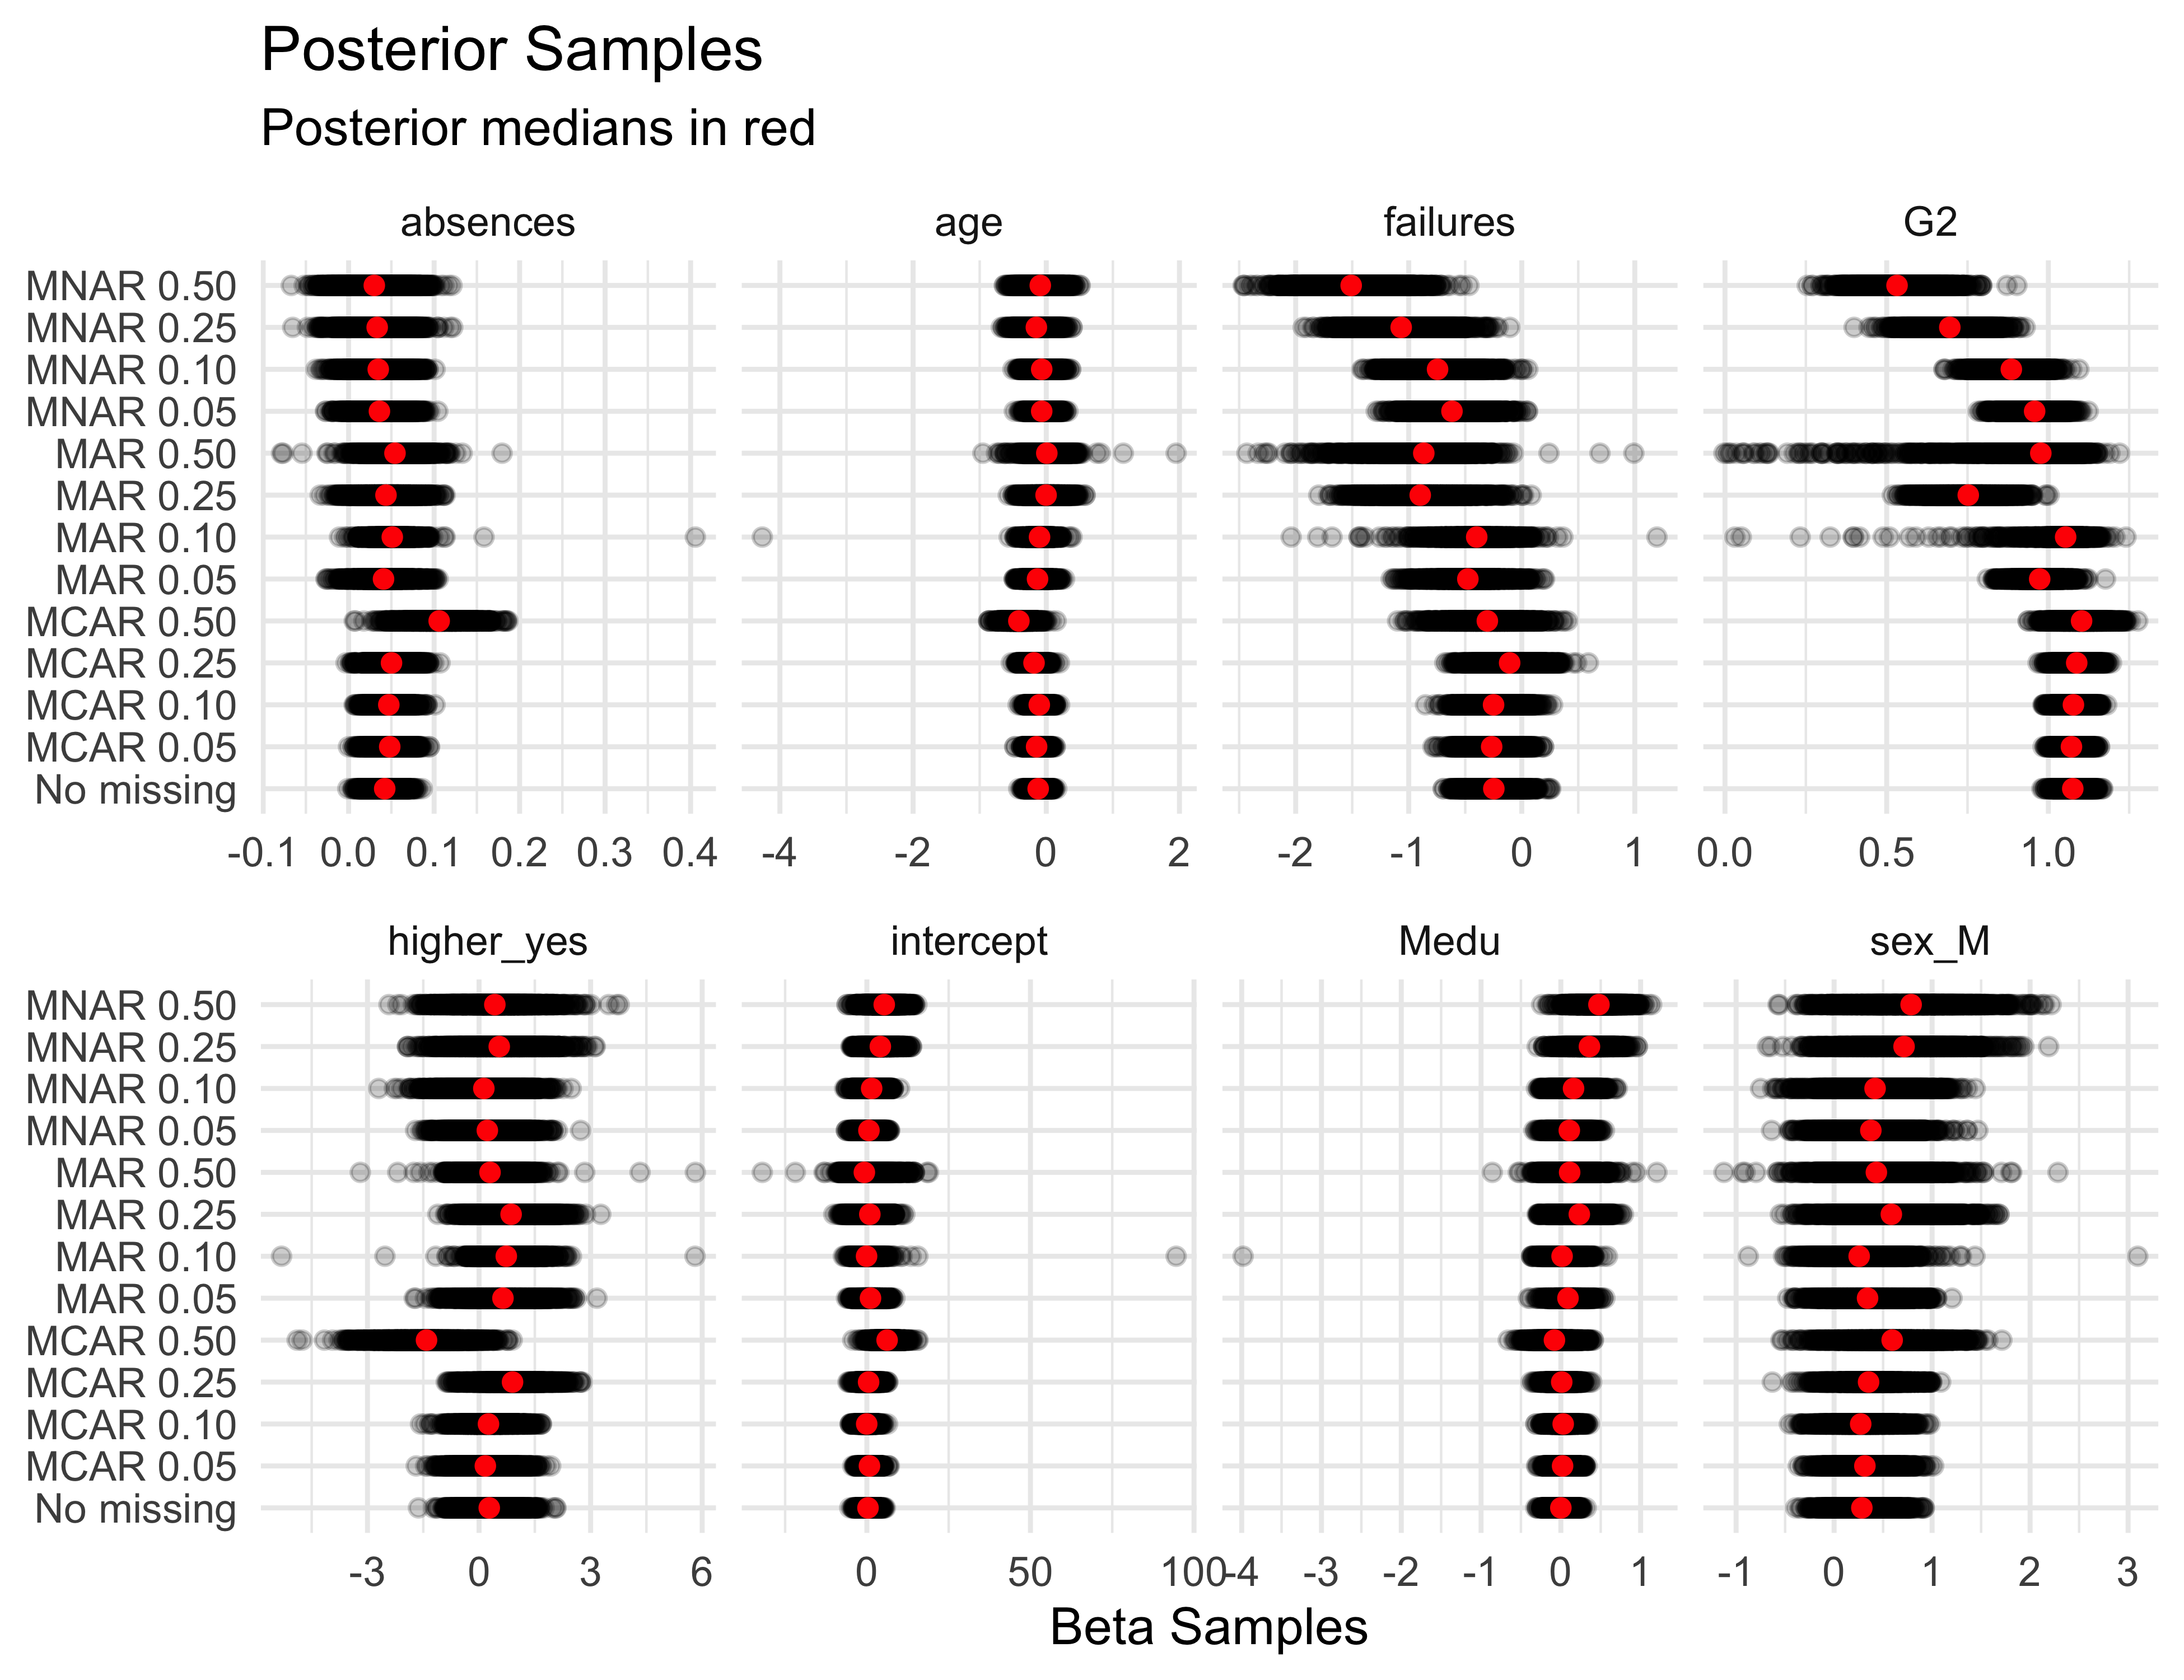
\includegraphics[width=6.5in, height=5in]{posterior-samples-1}

\textbf{Figure 2}

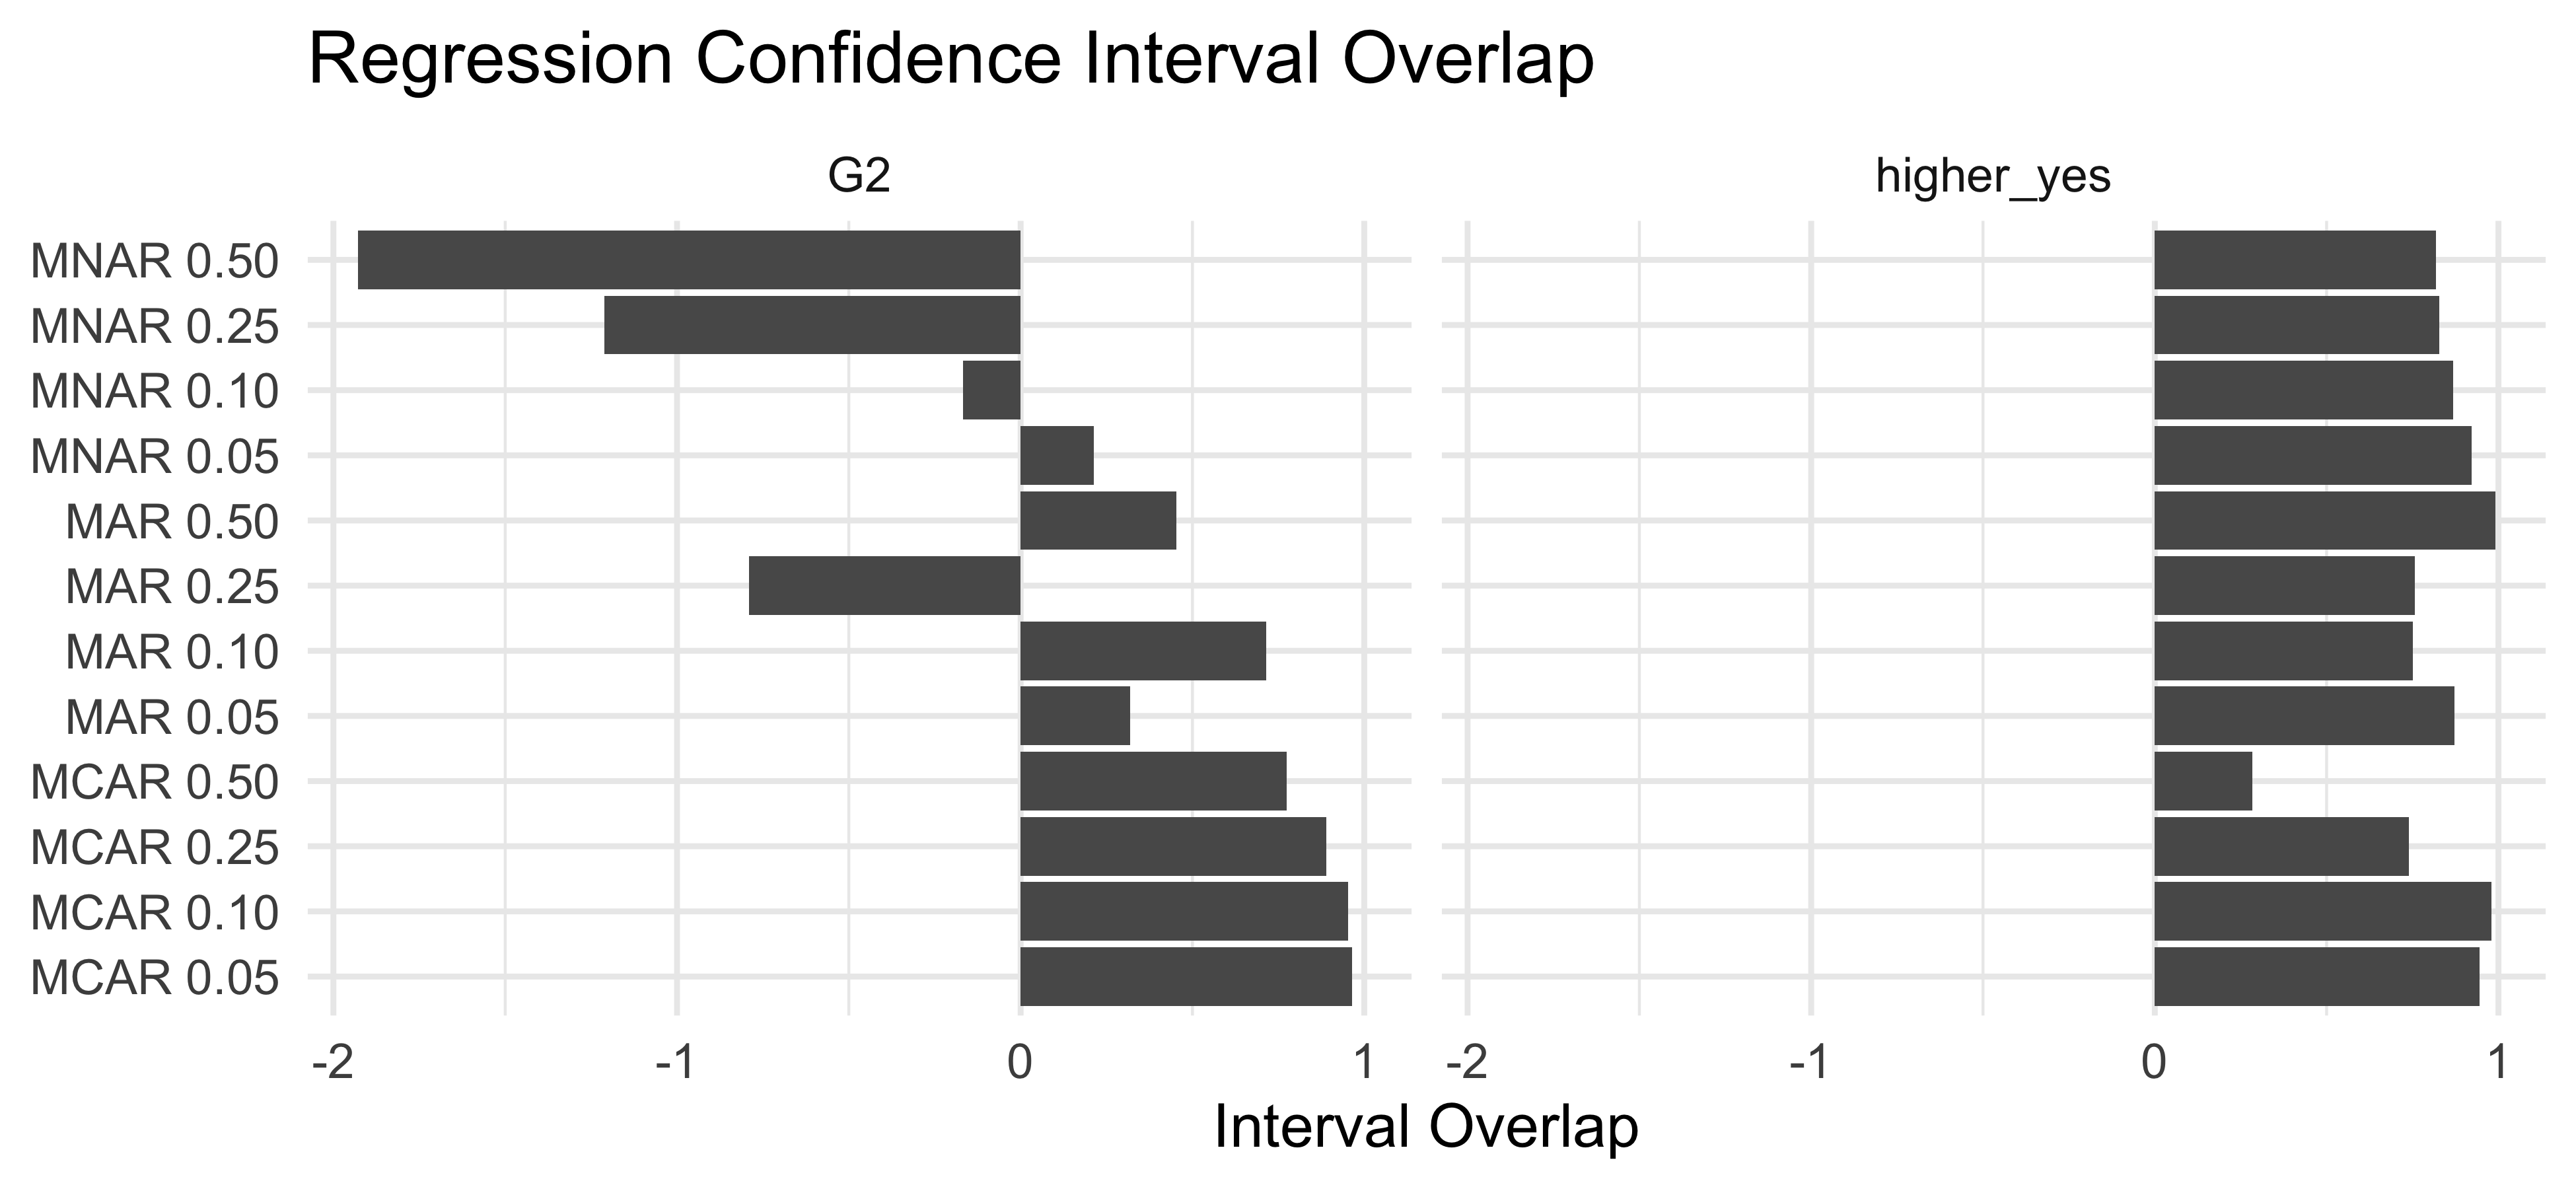
\includegraphics[width=6.5in, height=3in]{credible-interval-overlap-1}

\textbf{Figure 3} Imputations for MNAR missing at a rate of 0.25

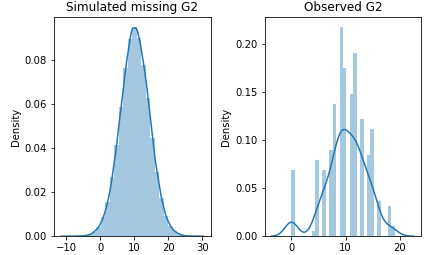
\includegraphics[width=4in, height=3in]{MNAR_025_G2}

\textbf{Figure 4} Imputations for MNAR missing at a rate of 0.25

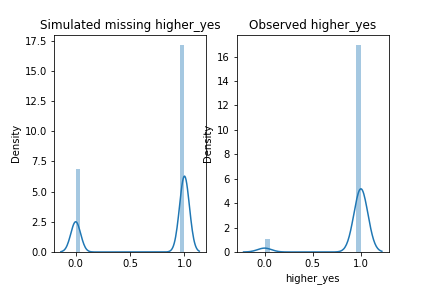
\includegraphics[width=4in, height=3in]{MNAR_025_higher_yes}

Further results are included in Appendix C. 

\section{Discussion}

Overall, the missing data methods are effective at mitigating the consequences of missing data; however, the effectiveness is based on extreme assumptions about the knowledge of the missingness and are very sensitive to the types and amount of missingness. 

Figure 1 plots the posterior samples and posterior median for each coefficient under each scenario. Bayesian linear regression without adjustment is robust to the MCAR missingness up to 50 percent even though we start with fewer than 400 observations. 

The MAR scenarios result in posterior samples with much greater variance for some coefficients, but the centers of the samples are for the most part accurate. The extra variance could be the result of the assumptions in the imputation model. Figure 5 in Appendix C shows that the inferences for most coefficients are the same too. Most of the coefficients have very small or very large effect sizes, so the inferences are only affected for age and failures.

The posterior samples for the MNAR scenario have less variance than the MAR scenarios but the posterior medians are very wrong for coefficients like failures and G2. Figure 2 shows that the 95 percent posterior credible intervals for G2 do not overlap at all in three of four MNAR situations. The weakness of the MAR methods is highlighted but its failure in the MNAR scenario in recreating the credible interval for the G2 coefficient.  

Figure 2 shows that the methods are very successful in all scenarios for the coefficient for higher\_yes. It is unclear if this is true of most binary variables or if it is because the variable is highly imbalanced and most values are "yes" as can be seen in Figure 4. For higher\_yes, the methods can't impute impossible values because the variable only takes on one of two levels. Figure 5 in Appendix C shows that for G2, which is continuous, the model did impute values outside of the range of the existing data. Figure 3 shows the density of the imputations as well as the density of the observed values. We also assume normality, which is approximately true but does not capture the spike of zero values in the true data. Assuming normality also carries the implication of allowing the entire real number line be the support for the variable G2. We know this is not true from the plot of observed G2 values in Figures 3 and 4. Further investigation into the data could suggest adding a latent variable for dropping the class and then modeling the data as normal conditional on staying in the class. The last thing to consider is that G2 dominates the model in importance. It would be interesting to see how these methods preform on more equal model coefficients.

\subsection{Further Research}

This simulation study demonstrates some properties of missing data methods, but more work could follow. The most obvious next step would be to directly model the missingness mechanism in the MNAR case. Following that, we could experiment with different starting points for the Gibbs sampler including multiple chains to improve the convergence of our parameters and imputations. We could experiment with different priors for the imputation model and the linear regression model of interest as we only used non-informative priors for the respective parameters. We could assume different imputation models for the respective variables with missing data. Finally, we could add missingness to more variables and experiment with dependence between the missingness since we manufactured independence into our missingness mechanisms here.

\newpage

\bibliography{references}
\bibliographystyle{apalike}

\newpage
\section{Appendix A}

The following definitions are mostly from \cite{gelman2021} but \cite{little2020} and \cite{vanBurren2018} were cited for clarity. 

\subsection{Definitions}

Let $y = (y_{obs}, y_{mis})$. Let $I$ be the inclusion indicator. Let $\theta$ be model parameters and let $\phi$ be parameters governing the missing data mechanism. Then the joint distribution of of interest is 

$$p(y, I|\theta, \phi) = p(y|\theta)p(I|y, \phi)$$

\vspace{0.25in}

\textbf{Definition:} \textit{inclusion indicator} -- A data structure with the same size and shape as as $y$ with 1 if the corresponding component is observed and 0 if the corresponding component is missing.

\vspace{0.25in}

\textbf{Definition:} \textit{inclusion model} -- The part of the statistical model that tries to model the inclusion indicator. The nature of this model is determined by the type of missingness. 

$$p(I|y_{obs}, y_{mis}, \phi)$$

\vspace{0.25in}

\textbf{Definition:} \textit{missing completely at random (MCAR)} -- If the probability of missingness is the same for all observations. Cause of missingness is unrelated to the data. A simple example is random sampling. This is also called \textit{observed at random}.

$$p(I|y_{obs}, y_{mis}, \phi) = p(I| \phi)$$

\vspace{0.25in}

\textbf{Definition:} \textit{missing at random (MAR)} -- If the distribution of the missing data mechanism does not depend on the missing values. \textit{The distribution of the missing data mechanism can depend on fully observed values in the data and parameters for the missing data mechanism.} A simple example is a stratified random sample. 

$$p(I|y_{obs}, y_{mis}, \phi) = p(I|y_{obs}, \phi)$$

\vspace{0.25in}

\textbf{Definition:} \textit{ignorable missing data mechanism} -- If the parameters for the missing data mechanism $\phi$ and the parameters for the model $\theta$ are distinct, then the missing data mechanism is said to be ignorable. (BDA frames this as $\phi$ and $\theta$ are independent in the prior distribution). 

$$p(y_{obs},I|\theta, \phi) = p(y_{obs}|\theta)$$

In this situation

$$p(\theta|x, y_{obs}) = p(\theta|x, y_{obs}, I)$$

\vspace{0.25in}

\textbf{Definition:} \textit{missing not at random (MNAR)} -- If the missing data mechanism depends on the missing values. Neither MCAR or MAR holds. The data are missing for reasons that are unknown to us. 

\vspace{0.5in}

\newpage
\section{Appendix B}

Below we explain the model setup as well as the sampling procedure used.

\subsubsection{Model Setup}

Let $y = (y_{mis}, y_{obs})$ and $\mathbf{X} = (\mathbf{X}_{mis}, \mathbf{X}_{obs})$

We assume the distribution of $\vec{Y}$ is

$$Y \sim MVN(\mathbf{X}\vec{\beta}, \sigma^2\mathbf{I})$$

We assume a non-informative prior with $\vec{\beta}$ with a flat prior and $\sigma^2$ with Jeffreys' prior

$$p(\vec{\beta}, \sigma^2) \propto (\sigma^2)^{-1}$$

\vspace{0.25in}

We include two imputation models. First, for missing values of G2, we assume a normal distribution such that

$$X_{G2} \sim MVN(\mathbf{X}_{Age}\vec{\gamma}, \eta^2\mathbf{I})$$

We assume a non-informative prior with $\vec{\gamma}$ with a flat prior and $\eta^2$ with Jeffreys' prior

$$p(\vec{\gamma}, \eta^2) \propto (\eta^2)^{-1}$$

\vspace{0.25in}

Second, for missing values of Higher, we assume a Bernoulli distribution and we use Normal approximation for logistic regression. So the likelihood $\mathcal{L}(y_i|x_i'\vec\alpha, \Phi)$ can be approximated by the normal likelihood $N(z_i, \theta^2_i)$.

\subsubsection{Sampling Procedure}

The sampling procedure is similar to an EM algorithm. There are imputation steps and then conditional posterior steps. We use the sample mean for G2, "Yes" for Higher (sample mode), and OLS estimates from the complete data for everything else for all starting values. The Gibbs sampler has the following steps:

\vspace{0.25in}

\textbf{Imputation step 1.} $X_{mis, G2}|\vec\gamma, \eta, X_{mis, Age}$

$$X_{mis, G2}^{(b)}|\vec\gamma^{(b - 1)}, \eta^{2(b - 1)}, X_{mis, Age} \sim MVN(\mathbf{X}\vec{\gamma}^{(b - 1)}, \eta^{2(b - 1)}\mathbf{I})$$

where $\mathbf{X}$ is a design matrix with $X_{Age}$.

This is derived on slides 169-173 in notes set 1.

\vspace{0.25in}

\textbf{Imputation step 2.} $X_{mis, Higher}|\alpha_0, \alpha_1, X_{mis, Age}$

$$X_{mis, Higher}^{(b)}|\vec\alpha^{(b - 1)}, X_{mis, Age} \sim Bernoulli\left(\frac{exp(\alpha_0 + \alpha_1X_{age})}{1 + exp(\alpha_0 + \alpha_1X_{age})}\right)$$

\textbf{Conditional posterior 1.} $\vec\beta | \sigma^2, y, \mathbf{X}$

$$\vec\beta^{(b)} | \sigma^{2(b - 1)}, y, \mathbf{X} \sim MVN((\mathbf{X}^T\mathbf{X})^{-1}\mathbf{X}^T\vec{Y}, \sigma^{2(b - 1)}(\mathbf{X}^T\mathbf{X}^{-1}))$$

where $\mathbf{X}$ is a design matrix with all predictors.

This is derived on slides 169-173 in notes set 1.

\vspace{0.25in}

\textbf{Conditional posterior 2.} $\sigma^2 | \vec\beta, y, \mathbf{X}$

$$\sigma^{2(b)} | \vec\beta^{(b - 1)}, y, \mathbf{X} \sim IG\left(\frac{n - k}{2}, \frac{1}{2}(\vec{Y} - \mathbf{X}\vec{\hat\beta^{(b - 1)}})^T(\vec{Y} - \mathbf{X}\vec{\hat\beta^{(b - 1)}})\right)$$

where $\mathbf{X}$ is a design matrix with all predictors.

This is derived on slides 169-173 in notes set 1.

\vspace{0.25in}

\textbf{Conditional posterior 3.} $\vec{\gamma}|\eta^2, X_{obs, G2}, X_{obs, Age}, X_{mis, G2}, X_{mis, Age}$

$$\vec{\gamma}^{(b)}|\eta^{2(b - 1)}, X_{obs, G2}, X_{obs, Age}, X_{mis, G2}, X_{mis, Age} \sim MVN((\mathbf{X}^T\mathbf{X})^{-1}\mathbf{X}^T\vec{X}_{G2}, \eta^{2(b - 1)}(\mathbf{X}^T\mathbf{X}^{-1}))$$

where $\mathbf{X}$ is a design matrix with $X_{Age}$.

This is derived on slides 169-173 in notes set 1.

\vspace{0.25in}

\textbf{Conditional posterior 4.} $\eta^2|\vec{\gamma}, X_{obs, G2}, X_{obs, Age}, X_{mis, G2}, X_{mis, Age}$

$$\eta^{2(b)}|\vec{\gamma}^{(b - 1)}, X_{obs, G2}, X_{obs, Age}, X_{mis, G2}, X_{mis, Age} \sim IG\left(\frac{n - k}{2}, \frac{1}{2}(\vec{X}_{G2} - \mathbf{X}\vec{\hat\gamma^{(b - 1)}})^T(\vec{X}_{G2} - \mathbf{X}\vec{\hat\gamma^{(b - 1)}})\right)$$

where $\mathbf{X}$ is a design matrix with $X_{Age}$.

This is derived on slides 169-173 in notes set 1.

\vspace{0.25in}

\textbf{Conditional posterior 5.} $\vec\alpha| \theta^2, X_{obs, Higher}, X_{obs, Age}, X_{mis, Higher}, X_{mis, Age}$

$$\vec\alpha^{(b)}|  X_{obs, Higher}, X_{obs, Age}, X_{mis, Higher}, X_{mis, Age} \dot\sim MVN(\hat{\vec\alpha}, V_{\alpha})$$

where $\hat{\vec\alpha}$ is the posterior mode found through Newton-Raphson and $V_{\alpha}$ is the last working variance from iterative solution to the posterior mode.

This is derived on slides 206-208 in notes set 1.

We note that once all relevant parameters are sampled, we discard some of these samples to account for burn-in and thinning per what we have seen in class.

\newpage

\section{Appendix C}

\textbf{Figure 3}

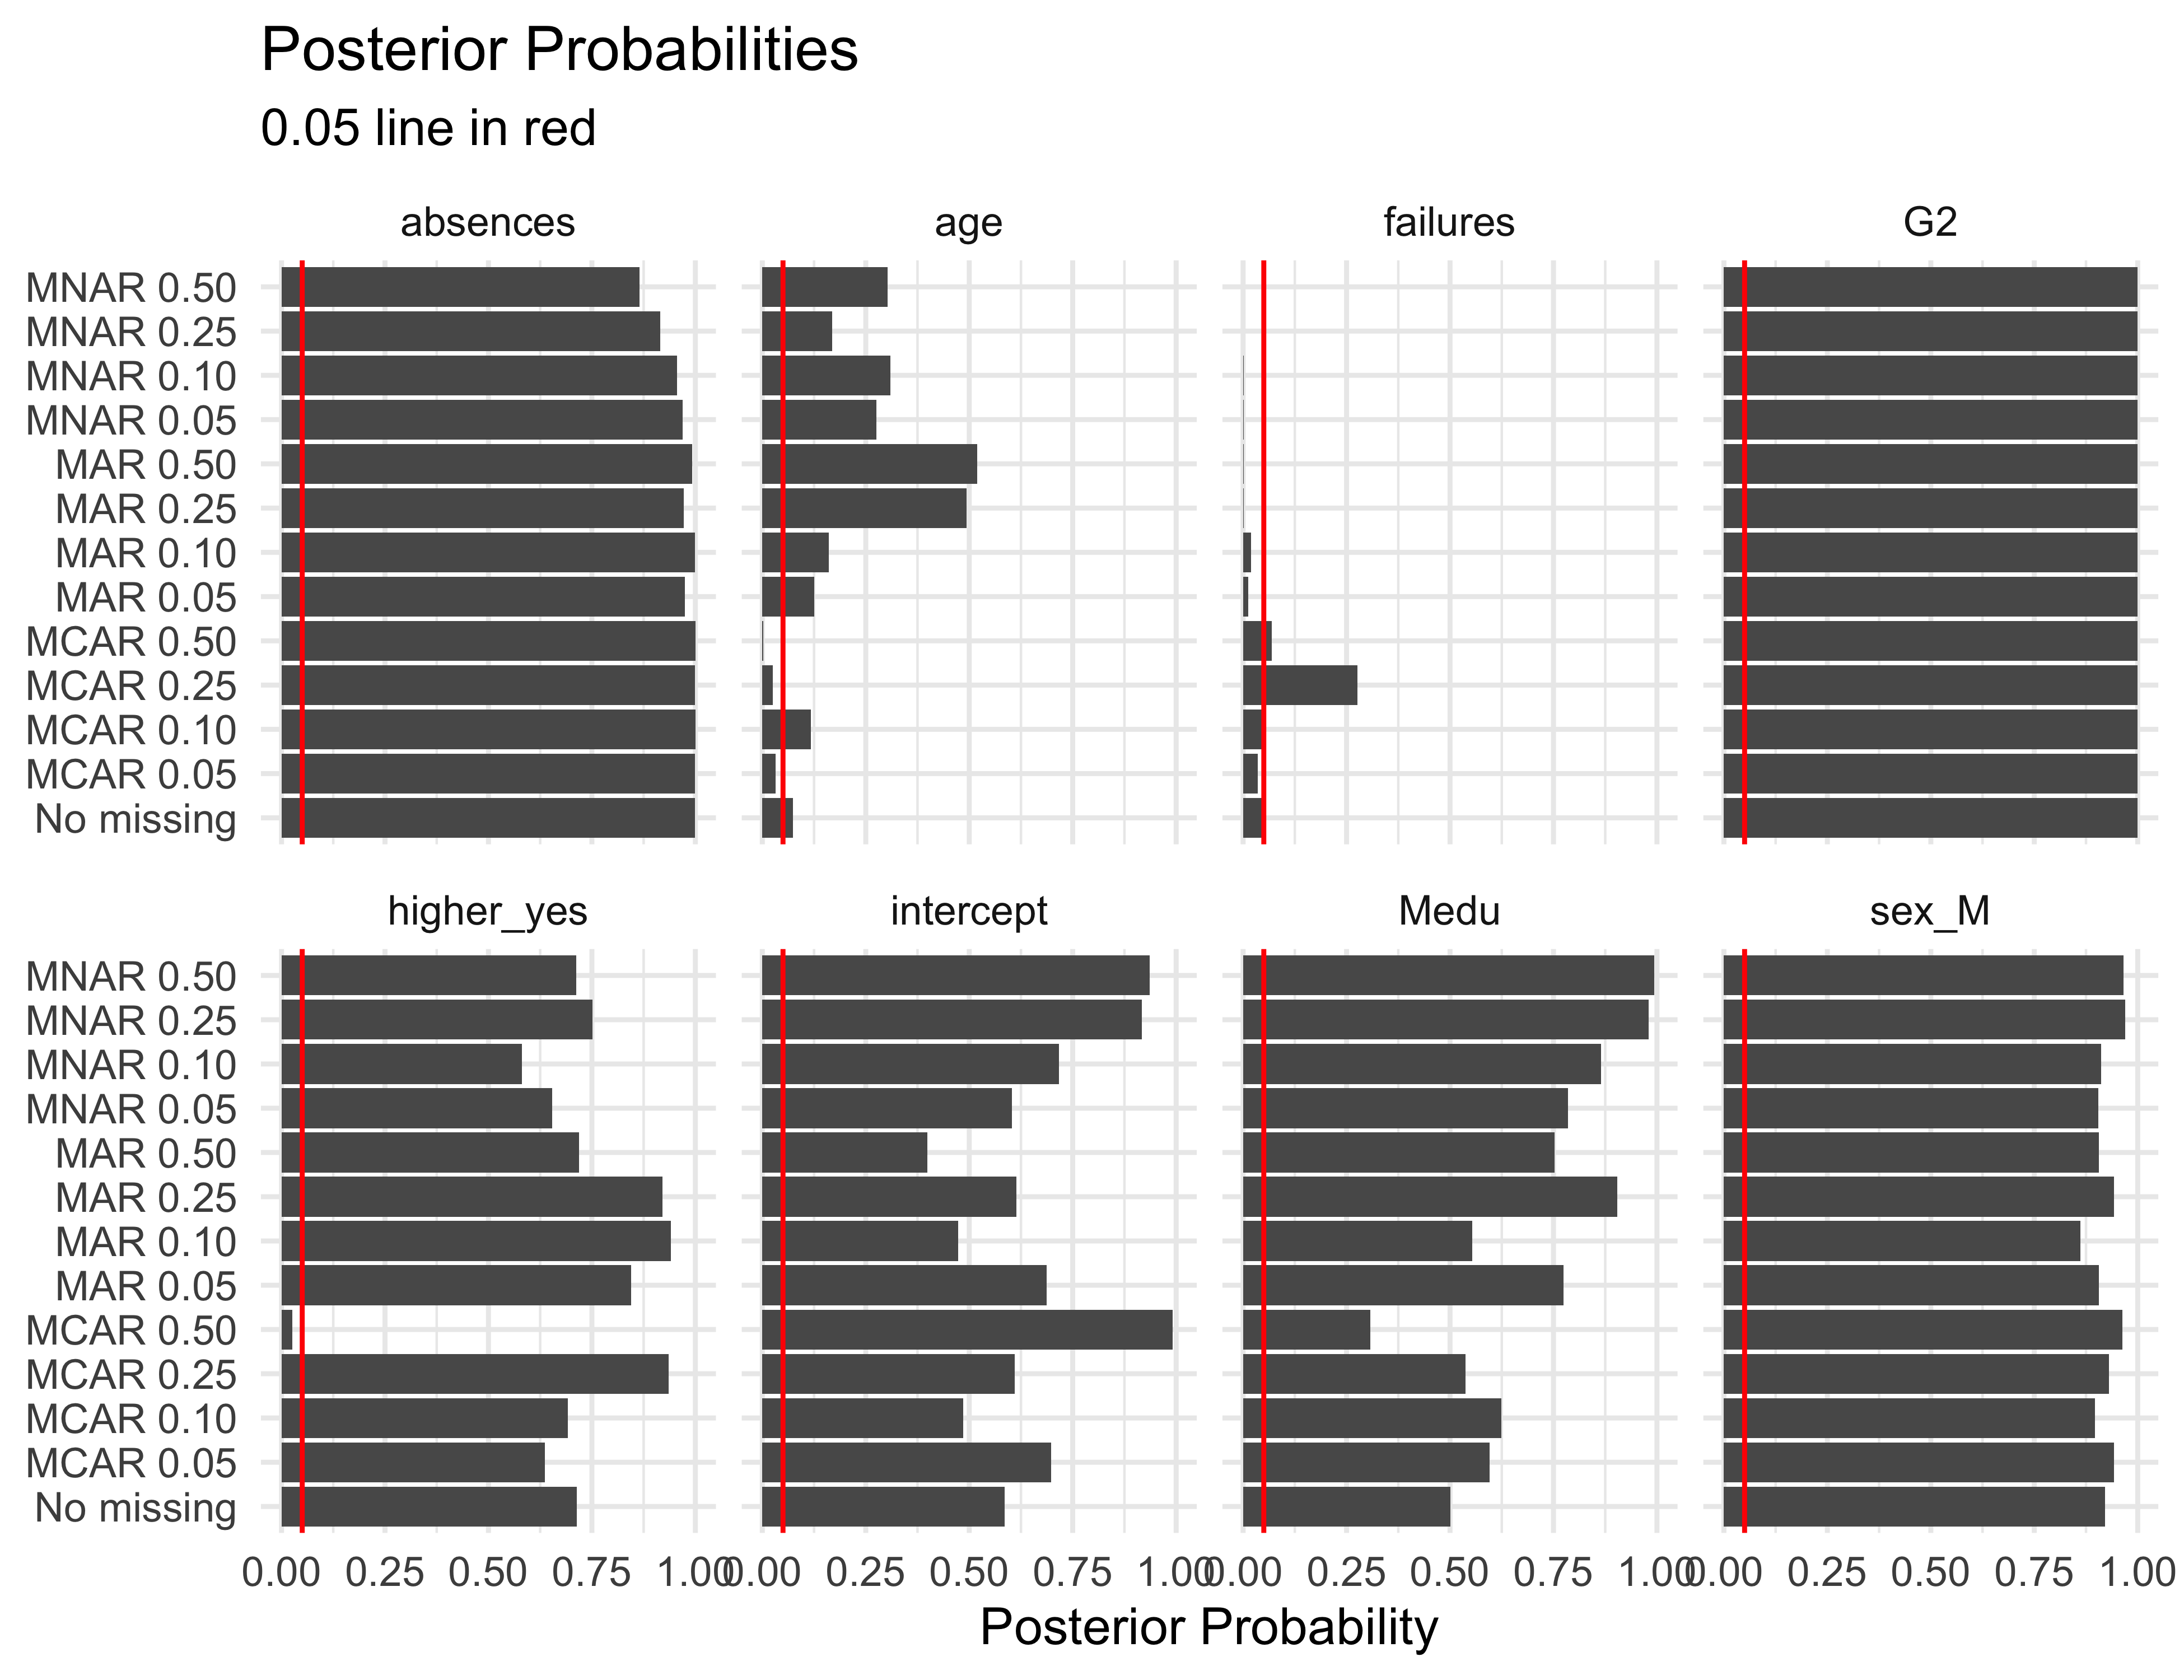
\includegraphics[width=6.5in, height=5in]{posterior-probabilities-1}

\textbf{Figure 4}

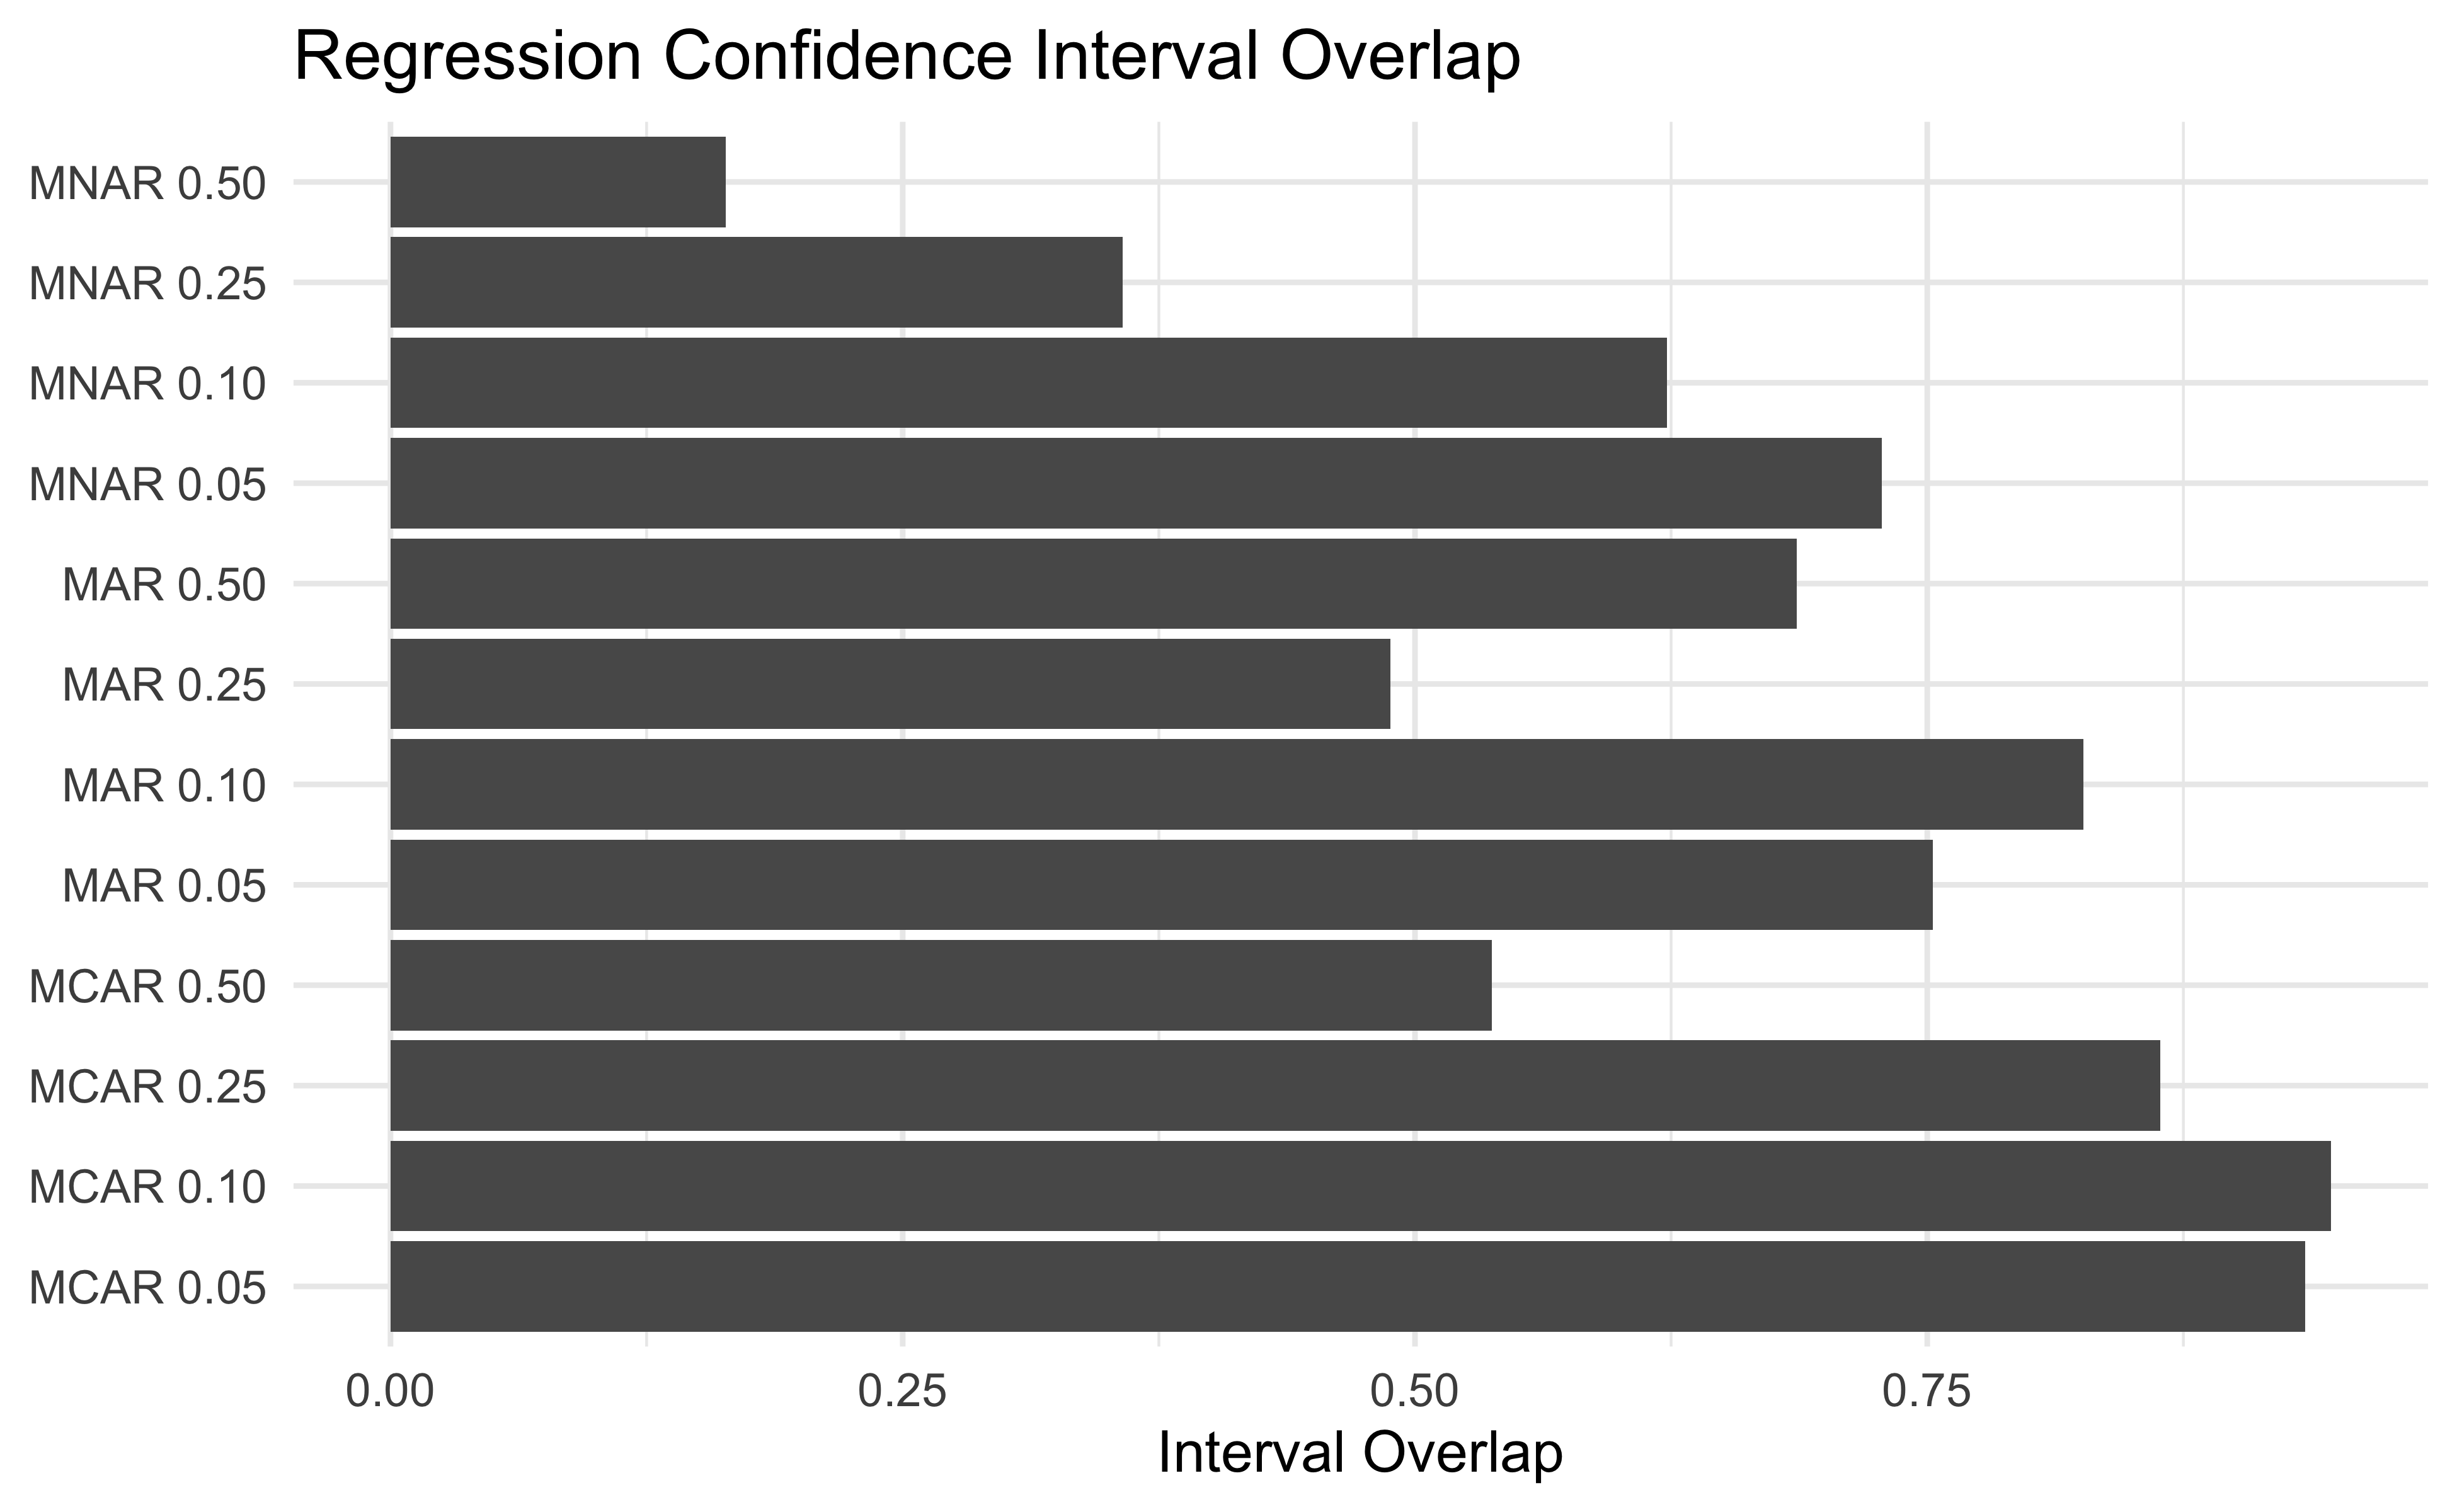
\includegraphics[width=6.5in, height=4in]{credible-interval-overlap-overall-1}



\end{document}




